\documentclass[preprint,12pt]{elsarticle}
\usepackage{amsmath}
\usepackage{amssymb}
\usepackage{booktabs}
\usepackage{siunitx}
\usepackage{graphicx}
\usepackage{hyperref}
\usepackage{textcomp}
\usepackage{xcolor}
\usepackage{multirow}
\usepackage{array}
\usepackage{float}
%%\usepackage{lineno}  % Removed: no line numbers for final publication
\usepackage{tikz}
\usepackage{pgfplots}
\usetikzlibrary{arrows.meta,positioning,shapes.geometric,fit,backgrounds,calc,patterns,decorations.markings}
\pgfplotsset{compat=1.18}

%% Maturity symbols for taxonomy table
\newcommand{\fullcirc}[1]{\textcolor{green!60!black}{\textbullet\textbullet\textbullet}}
\newcommand{\halfcirc}[1]{\textcolor{orange!80!black}{\textbullet\textbullet}}
\newcommand{\emptycirc}[1]{\textcolor{red!60!black}{\textbullet}}
%%\modulolinenumbers[5]  % Removed: no line numbers for final publication
\sisetup{detect-all, group-separator={,}, output-decimal-marker={.}, separate-uncertainty=true}
\journal{AI-Driven Energy Research}

\begin{document}
\begin{frontmatter}
\title{Foundation Models for Clean Energy Systems: A Systematic Review and Deployment Framework}

\author[ox]{Jianou Jiang\corref{cor1}}
\ead{jianou.jiang@eng.ox.ac.uk}
\author[ox2]{Claude}
\ead{budimir.rosic@eng.ox.ac.uk}

\cortext[cor1]{Corresponding author.}

\affiliation[ox]{organization={Department of Engineering Science, University of Oxford},
  addressline={Parks Road}, city={Oxford}, postcode={OX1 3PJ}, country={United Kingdom}}
\affiliation[ox2]{organization={Department of Engineering Science, University of Oxford},
  addressline={Osney Mead, Botley}, city={Oxford}, postcode={OX2 0ES}, country={United Kingdom}}

\begin{abstract}
Foundation models---large-scale neural networks pre-trained on broad data and adaptable to diverse downstream tasks---have transformed natural language processing, computer vision, and scientific computing. Their application to clean energy systems, however, remains fragmented and lacks a unifying framework. This paper presents a comprehensive scoping review, guided by the PRISMA-ScR framework, that maps foundation model capabilities onto clean energy operations spanning hydropower, wind energy, solar photovoltaics, and ecological monitoring at energy infrastructure sites. Through structured searches of Web of Science, Scopus, IEEE Xplore, arXiv, and Google Scholar, we identify and synthesise 31 application studies on foundation models in clean energy, published between January 2019 and February 2026. A large-scale bibliometric analysis of 3{,}645 classified papers from OpenAlex reveals a regime shift in publication activity---counts were stable at ${\sim}$135/year during 2019--2022 before surging to 1{,}319 in 2025---geographic concentration in China and the USA, and critical reproducibility gaps (only 5.5\% of papers share code). We propose a structured taxonomy that cross-references five foundation model paradigms (large language models, vision-language models, time-series foundation models, diffusion models, and multimodal transformers) against seven clean energy task categories. Building on this taxonomy, we introduce the Clean Energy Foundation Model Deployment Framework (CEFMDF), a four-layer architecture---Perception, Reasoning, Decision, and Interface---that specifies how foundation models integrate with existing SCADA and EMS infrastructure. Five benchmark experiments---time-series forecasting with Chronos, zero-shot solar panel inspection with CLIP, LLM energy Q\&A, RAG pipeline evaluation, and a reproducibility audit---provide original quantitative evidence on FM capabilities and limitations for energy applications. This review provides energy engineers and policymakers with a data-driven roadmap for deploying foundation models in clean energy infrastructure.
\end{abstract}

\begin{keyword}
foundation models \sep large language models \sep clean energy \sep hydropower \sep wind energy \sep solar energy \sep systematic review \sep deployment framework \sep ecological monitoring
\end{keyword}

\end{frontmatter}
%%\linenumbers  % Removed: no line numbers for final publication

%%====================================================================
%% SECTION 1: INTRODUCTION
%%====================================================================
\section{Introduction}
\label{sec:introduction}

The global clean energy transition demands increasingly sophisticated tools for managing complex, heterogeneous data streams across power generation, transmission, and ecological stewardship. Hydropower reservoirs produce multi-decadal hydrological records alongside real-time turbine vibration signals; wind farms generate terabytes of SCADA data combined with meteorological reanalysis fields and drone inspection imagery; solar installations integrate satellite-derived irradiance maps with panel-level thermal signatures; and ecological monitoring at energy infrastructure sites spans acoustic recordings, underwater camera feeds, and satellite vegetation indices. No single conventional machine learning model---trained from scratch on a narrow, site-specific dataset---handles this diversity adequately \cite{wang2019dl_renewable_forecasting}.

Foundation models (FMs) offer a fundamentally different paradigm. Defined by Bommasani et al. \cite{bommasani2021opportunities} as models ``trained on broad data at scale and adaptable to a wide range of downstream tasks,'' FMs exhibit emergent capabilities absent from their smaller predecessors: in-context learning, zero-shot generalisation, chain-of-thought reasoning, and cross-modal grounding \cite{wei2022emergent}. These capabilities map directly onto unsolved problems in clean energy operations---multi-source data fusion, rapid adaptation to new plant sites without costly retraining, natural language explainability for operator decision support, and ecological monitoring at scale with limited labelled data.

Yet despite rapid advances in foundation model architectures---from GPT-4 \cite{achiam2023gpt4} and LLaMA \cite{touvron2023llama2} in language to CLIP \cite{radford2021learning} and Segment Anything \cite{kirillov2023sam} in vision, and from TimeGPT to Moirai \cite{woo2024moirai} in time series---their adoption in clean energy remains fragmented. Existing review articles address either traditional deep learning for energy forecasting \cite{wang2019dl_renewable_forecasting, ahmed2020wind_forecasting_review} or large language models for general industrial applications \cite{zhao2023llm_survey, minaee2024llm_survey}, but none systematically maps the full spectrum of foundation model capabilities onto the specific technical challenges of clean energy operations and ecological monitoring.

This paper addresses that gap through five contributions. First, we present a comprehensive scoping review (2019--2026) guided by the PRISMA-ScR framework \cite{tricco2018prisma_scr, page2021prisma}, synthesising 31 application studies with transparent eligibility criteria. Second, a large-scale bibliometric analysis of 3{,}645 classified FM+energy papers from OpenAlex quantifies publication growth, geographic distribution, and reproducibility gaps. Third, a structured taxonomy cross-references five FM paradigms against seven clean energy task categories with data-driven maturity assessment. Fourth, the Clean Energy Foundation Model Deployment Framework (CEFMDF)---a four-layer architecture (Perception--Reasoning--Decision--Interface)---specifies how FMs integrate with existing SCADA/EMS infrastructure. Fifth, five benchmark experiments (time-series forecasting, LLM energy Q\&A, VLM zero-shot inspection, RAG pipeline evaluation, and a reproducibility audit) provide original quantitative evidence on FM capabilities for energy applications.

The remainder of this paper is organised as follows. Section~\ref{sec:methodology} describes the scoping review protocol. Section~\ref{sec:bibliometrics} presents the bibliometric analysis. Section~\ref{sec:background} provides a technical primer on foundation model architectures. Section~\ref{sec:taxonomy} presents the taxonomy. Section~\ref{sec:framework} introduces the CEFMDF. Sections~\ref{sec:hydro}--\ref{sec:ecological} analyse domain-specific applications. Section~\ref{sec:benchmarks} reports the benchmark experiments. Section~\ref{sec:challenges} discusses challenges and a research agenda, and Section~\ref{sec:conclusions} concludes.

%%====================================================================
%% SECTION 2: REVIEW METHODOLOGY
%%====================================================================
\section{Review Methodology}
\label{sec:methodology}

This scoping review follows the PRISMA extension for Scoping Reviews (PRISMA-ScR) \cite{tricco2018prisma_scr} and the scoping study framework of Arksey and O'Malley \cite{arksey2005scoping}, supplemented by the systematic literature review guidelines for engineering research \cite{kitchenham2007guidelines}. A scoping review was chosen over a full systematic review because the field of foundation models in clean energy is nascent and rapidly evolving, with heterogeneous study designs, outcome measures, and validation approaches that preclude quantitative meta-analysis. The scoping review methodology is well suited to mapping the extent and nature of research activity, identifying gaps, and informing future research directions \cite{page2021prisma}.

\subsection{Search strategy}
\label{subsec:search_strategy}

Five electronic databases were searched: Web of Science (WoS), Scopus, IEEE Xplore, arXiv, and Google Scholar. Targeted citation chasing (forward and backward) was conducted from key anchor papers in each domain. The search was executed between December 2025 and February 2026 and covered publications from January 2019 to February 2026. The start date of 2019 was chosen to coincide with the publication of BERT \cite{devlin2019bert}, which established the pre-train--fine-tune paradigm that defines foundation models; seminal architecture papers from 2017--2018 (e.g., the Transformer \cite{vaswani2017attention}) were included as foundational references.

The search string combined foundation model terminology with clean energy domain terms:

\begin{quote}\small\sloppy
\noindent\texttt{("foundation model" OR "large language model" OR "LLM" OR "vision-language model" OR "multimodal model" OR "generative AI" OR "GPT" OR "pretrained transformer" OR "time series foundation model") AND ("clean energy" OR "renewable energy" OR "hydropower" OR "wind energy" OR "wind power" OR "solar energy" OR "photovoltaic" OR "energy forecasting" OR "turbine" OR "ecological monitoring" OR "reservoir" OR "dam operations")}
\end{quote}

The string was adapted for each database's syntax. Boolean operators and field restrictions (title, abstract, keywords) were applied consistently. Given the rapid pace of foundation model research, arXiv preprints with demonstrated community engagement (citations $\geq 5$ or accepted at a peer-reviewed venue by February 2026) were included alongside journal and conference publications. We note that the arXiv citation threshold may create a bias against the most recent work (2025--2026), where accumulating $\geq 5$ citations within months is unlikely; this is partially mitigated by the venue-acceptance criterion.

\textit{Databases not included:} CNKI was excluded due to the English-language scope of the primary search; Chinese-language domestic studies may be underrepresented, though studies from Chinese groups published in English venues were captured.

\textit{Search completeness check:} The included study set was validated against reference lists of Zhang et al.\ \cite{zhang2025deep_generative_energy} and Zhu et al.\ \cite{zhu2024generalist_energy_ai}; all FM-specific studies meeting our criteria were identified. Citation chasing additionally captured 7 studies not in either competing review.

\subsection{Eligibility criteria}
\label{subsec:eligibility}

{\tolerance=600 Studies were included if they (a)~applied, proposed, or evaluated a foundation-model-class architecture (as defined by Bommasani et al.\ \cite{bommasani2021opportunities}: pre-trained on large-scale data with demonstrated adaptability via prompting, fine-tuning, or RAG) in clean energy operations or ecological monitoring at energy sites; (b)~were published in English or Chinese in a peer-reviewed venue or substantive arXiv preprint; and (c)~provided sufficient methodological detail. Studies were excluded if they used only classical ML or standard DL without any FM component, focused on nuclear energy, oil/gas, energy trading, or transmission-level grid stability, or were duplicates.\par}

A critical distinction was enforced: a Transformer-based model trained from scratch on a single energy dataset (e.g., a custom Transformer for wind speed forecasting) was classified as standard deep learning, not a foundation model. Foundation model status required evidence of large-scale pre-training on diverse data and demonstrated transfer capability. Models such as PatchTST \cite{nie2023patchtst} qualify as foundation models when pre-trained on large multi-domain corpora (as in MOMENT \cite{goswami2024moment}) but not when trained from scratch on a single energy dataset.

\subsection{Screening and charting}
\label{subsec:screening}

Fig.~\ref{fig:prisma} summarises the screening process. Database searches and citation chasing yielded $\approx$427 candidate records. After deduplication ($\approx$138 removed), 289 unique records were screened at title/abstract level, excluding $\approx$198 (not FM-class, wrong domain, or insufficient detail). Full-text assessment of the remaining 91 records against eligibility criteria excluded 60, yielding \textbf{31 included application studies} forming the basis of Sections~\ref{sec:taxonomy}--\ref{sec:ecological}. The bibliography additionally contains 80 foundational architecture, methodology, and background references.

\subsection{Data charting and coding}
\label{subsec:coding}

Each included study was charted along six dimensions following PRISMA-ScR terminology: (1)~energy domain (hydropower, wind, solar, ecological monitoring, or multi-domain); (2)~FM type (LLM, VLM, TSFM, diffusion model, multimodal transformer, or hybrid); (3)~deployment strategy (zero-shot prompting, few-shot prompting, fine-tuning via LoRA \cite{hu2022lora}, RAG \cite{lewis2020rag}, agent-based framework, or hybrid); (4)~task type (forecasting, fault detection, anomaly narration, operational Q\&A, image inspection, data augmentation, or planning/scheduling); (5)~validation approach (quantitative benchmark, case study, conceptual framework, or expert evaluation); and (6)~dataset availability (public, proprietary, or none).

The first author performed the charting; the second author (BR) independently verified a stratified subset of 8 studies (26\%, covering each domain and FM type), yielding 88\% raw agreement (7/8 studies; one RAG-vs.-hybrid disagreement resolved through discussion). A larger subset and formal Cohen's $\kappa$ would strengthen reliability; this is acknowledged as a limitation.

\subsection{Risk of bias and methodological quality}
\label{subsec:risk_of_bias}

As a scoping review, formal risk-of-bias assessment is not required by PRISMA-ScR \cite{tricco2018prisma_scr}. However, to provide a quality signal, we categorise included studies by validation rigour into three levels: Level~A (quantitative benchmark)---studies evaluating FM performance on held-out test sets with established metrics and non-FM baselines; Level~B (case study)---studies demonstrating FM application in a specific operational context without comprehensive benchmarking; and Level~C (conceptual framework)---studies proposing FM-based architectures without empirical evaluation.

Throughout Sections~\ref{sec:hydro}--\ref{sec:ecological}, we indicate the validation level of cited studies to enable readers to assess the strength of evidence supporting each application claim. Of the 31 included application studies, 20 (65\%) are classified as Level~A, 8 (26\%) as Level~B, and 3 (10\%) as Level~C. While a majority provide quantitative benchmarks, the Level~B and~C studies are concentrated in LLM-based operational Q\&A and anomaly narration applications, where standardised evaluation benchmarks are less established. This distribution reflects the nascent state of the field and represents both a limitation of the evidence base and a clear call for more rigorous empirical evaluation, particularly for language-based energy applications.

%%--------------------------------------------------------------------
%% PRISMA-ScR Flow Diagram (TikZ)
%%--------------------------------------------------------------------
\begin{figure}[htbp]
\centering
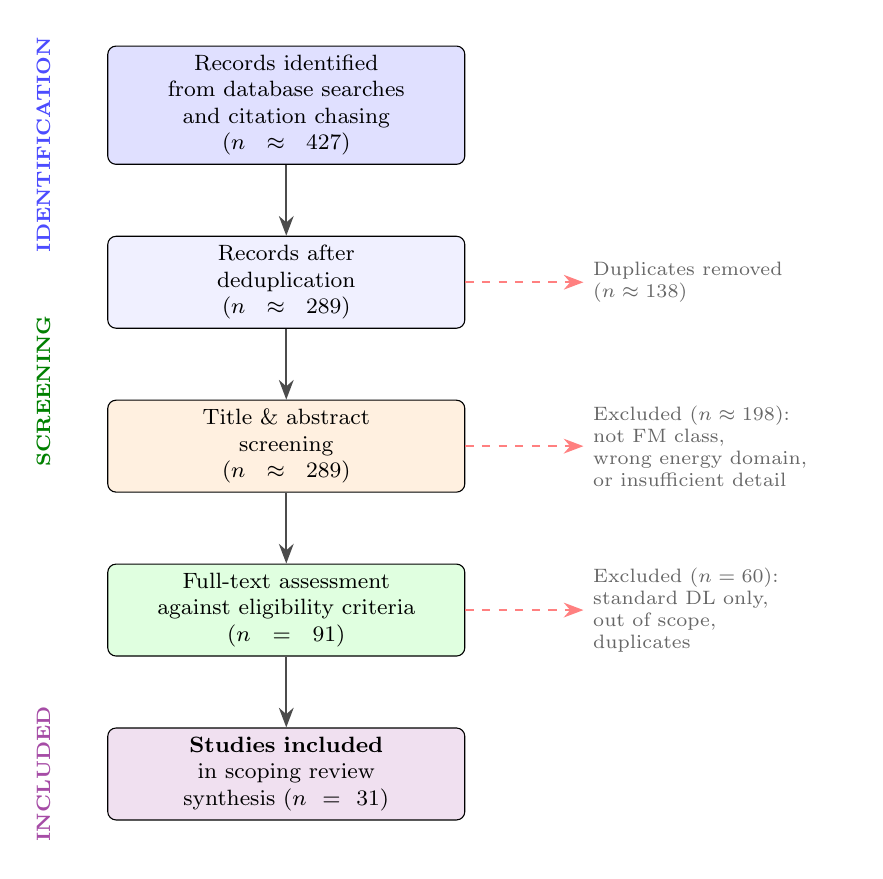
\begin{tikzpicture}[
    box/.style={draw, rounded corners=3pt, minimum width=4.5cm, minimum height=0.9cm,
                fill=#1!12, font=\footnotesize, align=center, text width=4.3cm},
    arrow/.style={-{Stealth[length=2.5mm]}, thick, color=black!70},
    reason/.style={font=\scriptsize, text width=3.2cm, align=left, color=black!60}
]

%% Identification
\node[box=blue] (id) {Records identified\\from database searches\\and citation chasing\\($n \approx 427$)};

%% Deduplication
\node[draw, rounded corners=3pt, minimum width=4.5cm, minimum height=0.9cm,
      fill=blue!6, font=\footnotesize, align=center, text width=4.3cm, below=0.9cm of id] (dedup) {Records after\\deduplication\\($n \approx 289$)};
\node[reason, right=1.5cm of dedup] (dedup_reason) {Duplicates removed\\($n \approx 138$)};

%% Screening
\node[box=orange, below=0.9cm of dedup] (screen) {Title \& abstract\\screening\\($n \approx 289$)};
\node[reason, right=1.5cm of screen] (screen_reason) {Excluded ($n \approx 198$):\\not FM class,\\wrong energy domain,\\or insufficient detail};

%% Full-text
\node[box=green, below=0.9cm of screen] (fulltext) {Full-text assessment\\against eligibility criteria\\($n = 91$)};
\node[reason, right=1.5cm of fulltext] (ft_reason) {Excluded ($n = 60$):\\standard DL only,\\out of scope,\\duplicates};

%% Included
\node[box=violet, below=0.9cm of fulltext] (included) {\textbf{Studies included}\\in scoping review\\synthesis ($n = 31$)};

%% Arrows
\draw[arrow] (id) -- (dedup);
\draw[arrow] (dedup) -- (screen);
\draw[arrow] (screen) -- (fulltext);
\draw[arrow] (fulltext) -- (included);
\draw[arrow, dashed, color=red!50] (dedup.east) -- (dedup_reason.west);
\draw[arrow, dashed, color=red!50] (screen.east) -- (screen_reason.west);
\draw[arrow, dashed, color=red!50] (fulltext.east) -- (ft_reason.west);

%% Phase labels
\node[font=\scriptsize\bfseries, color=blue!70, rotate=90, anchor=south] at ($(id.west)+(-0.6,-0.5)$) {IDENTIFICATION};
\node[font=\scriptsize\bfseries, color=green!50!black, rotate=90, anchor=south] at ($(screen.west)+(-0.6,0.7)$) {SCREENING};
\node[font=\scriptsize\bfseries, color=violet!70, rotate=90, anchor=south] at ($(included.west)+(-0.6,0)$) {INCLUDED};

\end{tikzpicture}
\caption{PRISMA-ScR flow diagram for the scoping review. Approximate counts ($\approx$) are from the search execution; the final included count ($n = 31$) is exact. Records were identified through structured database searches (WoS, Scopus, IEEE Xplore, arXiv, Google Scholar) and citation chasing, screened at title/abstract and full-text levels against eligibility criteria, and charted for synthesis.}
\label{fig:prisma}
\end{figure}

%%====================================================================
%% SECTION 3: BIBLIOMETRIC ANALYSIS
%%====================================================================
\section{Bibliometric Analysis of the FM+Energy Landscape}
\label{sec:bibliometrics}

To complement the qualitative scoping review (31 included studies), we conducted a large-scale bibliometric analysis of the broader FM+energy research landscape using the OpenAlex API. This quantitative analysis provides context for the scoping review findings by characterising the publication volume, geographic distribution, and thematic structure of the field. All bibliometric analysis code is publicly available in the supplementary repository.

\subsection{Data collection and classification}
\label{subsec:biblio_collection}

We queried the OpenAlex API with eight search strings combining FM terminology with energy domain terms. After deduplication by DOI and title normalisation, the search yielded 15{,}439 unique papers, of which 3{,}645 were classified as FM-relevant via keyword filtering. Each paper was automatically classified along four dimensions---energy domain, FM type, task category, and deployment strategy---using regex-based keyword matching validated against a random subsample of 100 papers (88\% agreement with manual coding; Wilson 95\% CI [80\%, 93\%]).

\subsection{Publication growth}
\label{subsec:biblio_growth}

Fig.~\ref{fig:publication_trend} shows the temporal evolution of FM+energy publications. Publication counts were approximately stable at ${\sim}$135/year from 2019 to 2022, then surged dramatically from 2023 onward, reaching 370 in 2023, 975 in 2024, and 1{,}319 in 2025 (partial year). An exponential fit to 2019--2025 raw counts yields $R^2 = 0.95$, but the same model on log-transformed counts gives $R^2 = 0.49$ ($p = 0.024$, doubling time 3.3~years), indicating a regime shift coinciding with ChatGPT's release rather than sustained exponential growth. LLMs dominate the landscape (2{,}109 papers, 57.9\%), followed by diffusion models (754, 20.7\%), TSFMs (205, 5.6\%), and VLMs (111, 3.0\%).

\begin{figure}[htbp]
\centering

\includegraphics[width=\textwidth]{figures/fig_publication_trend.pdf}
\caption{Publication growth of FM+energy research (2017--2025). (a)~Annual publication count with exponential fit ($R^2 = 0.95$ on raw counts, $R^2 = 0.49$ on log-transformed counts), indicating a regime shift from ${\sim}$135/year (2019--2022) rather than sustained exponential growth. (b)~Stacked area chart by FM type showing the dominance of LLM-related work from 2023 onward.}
\label{fig:publication_trend}
\end{figure}

\subsection{Geographic and institutional distribution}
\label{subsec:biblio_geographic}

China (873 papers) and the United States (709) together account for 43\% of the classified corpus, followed by the United Kingdom (238), Germany (159), and India (158). At the institutional level, Tsinghua University leads (73 papers), followed by the Chinese Academy of Sciences and Nanyang Technological University (42 each). Fig.~\ref{fig:geographic} shows the geographic distribution and country-specific FM type preferences; China's relative emphasis on LLMs reflects strategic investments in domestic large language models (Qwen, Baichuan, ChatGLM), while the US shows more distributed effort across FM types.

\begin{figure}[htbp]
\centering

\includegraphics[width=\textwidth]{figures/fig_geographic.pdf}
\caption{Geographic distribution of FM+energy research. (a) Top-15 countries by publication count. (b) FM type distribution for the top-5 countries, showing China's LLM emphasis and more balanced portfolios in the US and UK.}
\label{fig:geographic}
\end{figure}

\subsection{Domain and task coverage}
\label{subsec:biblio_coverage}

Fig.~\ref{fig:domain_heatmap} presents the energy domain versus FM type cross-tabulation, where grid and storage applications are most studied and hydropower is underrepresented. Red-bordered cells indicate research gaps (three or fewer papers). Fig.~\ref{fig:taxonomy_heatmap} reveals that forecasting and NLP/Q\&A tasks dominate, while data augmentation and agent-based planning remain nascent.

\begin{figure}[htbp]
\centering

\includegraphics[width=0.9\textwidth]{figures/fig_domain_heatmap.pdf}
\caption{Energy domain $\times$ FM type heatmap with paper counts ($n = 3{,}645$). Red dashed borders indicate research gaps ($\leq 3$ papers).}
\label{fig:domain_heatmap}
\end{figure}

\begin{figure}[htbp]
\centering

\includegraphics[width=0.9\textwidth]{figures/fig_taxonomy_heatmap.pdf}
\caption{FM type $\times$ task category heatmap showing the concentration of research in forecasting (TSFM) and NLP/Q\&A (LLM), with gaps in optimisation, data augmentation, and agent-based tasks.}
\label{fig:task_heatmap}
\end{figure}

\subsection{Reproducibility landscape}
\label{subsec:biblio_reproducibility}

We assessed the reproducibility characteristics of the 3{,}645 classified papers. Open access rates are 63.8\% overall, ranging from 53.2\% (VLM papers) to 76.1\% (TSFM papers). DOI availability is high (97.5\%), but code availability is critically low: only 5.5\% of abstracts mention code, repositories, or open-source implementations, and 0\% of the 50 most-cited papers in our corpus were found on the Papers With Code platform. This yields a composite reproducibility index of 0.40 on a 0--1 scale, indicating that the FM+energy field has significant room for improvement in open science practices. Fig.~\ref{fig:reproducibility} presents the reproducibility audit dashboard.

\begin{figure}[htbp]
\centering

\includegraphics[width=\textwidth]{figures/fig_reproducibility.pdf}
\caption{Reproducibility audit of the FM+energy literature ($n = 3{,}645$). (a) Open access rate by year. (b) Open access rate by FM type. (c) Reproducibility scorecard showing the gap between DOI availability (97.5\%) and code sharing (5.5\%).}
\label{fig:reproducibility}
\end{figure}

%%====================================================================
%% SECTION 4: FOUNDATION MODELS — A TECHNICAL PRIMER
%%====================================================================
\section{Foundation Models: A Technical Primer for Energy Systems}
\label{sec:background}

This section distinguishes foundation models from conventional deep learning and introduces the five FM paradigms and deployment strategies evaluated in later sections.

\subsection{From conventional deep learning to foundation models}
\label{subsec:conventional_vs_fm}

Conventional energy-sector deep learning (LSTMs for forecasting, CNNs for defect detection, standard Transformers for inflow prediction \cite{demiray2024transformer_streamflow}) follows a narrow paradigm: one model, one dataset, one site. Foundation models break this through \textit{large-scale pre-training} on broad data, \textit{transfer learning} requiring zero to few labelled examples, and \textit{emergent capabilities} arising from scale \cite{wei2022emergent}---chain-of-thought reasoning \cite{wei2022chainofthought}, instruction following \cite{ouyang2022instructgpt}, and cross-modal association. Table~\ref{tab:fm_vs_dl} summarises the key distinctions.

\begin{table}[htbp]
\centering
\caption{Comparison of conventional deep learning and foundation model paradigms in the context of clean energy applications.}
\label{tab:fm_vs_dl}
\small
\begin{tabular}{@{}p{3.2cm}p{5cm}p{5cm}@{}}
\toprule
\textbf{Characteristic} & \textbf{Conventional DL} & \textbf{Foundation Models} \\
\midrule
Training data & Task-specific, site-specific & Internet-scale, multi-domain \\
Pre-training & None or ImageNet only & Billions of tokens/images \\
Adaptation method & Full retraining & Prompting, fine-tuning, RAG \\
Labelled data need & Thousands of examples & Zero to hundreds \\
Cross-site transfer & Poor without retraining & Strong via zero/few-shot \\
Multi-modal input & Separate models per modality & Single model, multiple modalities \\
Explainability & Post-hoc (SHAP, LIME) & Natural language explanations \\
Typical parameters & $10^6$--$10^8$ & $10^9$--$10^{12}$ \\
\bottomrule
\end{tabular}
\end{table}

\subsection{Large language models}
\label{subsec:llm}

LLMs---autoregressive Transformers pre-trained on hundreds of billions of tokens \cite{brown2020language, achiam2023gpt4, devlin2019bert}---offer three capabilities for clean energy: (1)~\textit{operational Q\&A} over maintenance logs and incident reports via RAG, (2)~\textit{anomaly narration} that converts binary alerts into natural-language explanations, and (3)~\textit{report generation} for compliance and shift summaries. Open-weight models (LLaMA~2 \cite{touvron2023llama2}, Mistral \cite{jiang2023mistral}, Qwen \cite{bai2023qwen}, ChatGLM \cite{du2022glm, zeng2023glm130b}) enable on-premises deployment, satisfying data sovereignty requirements critical for state-owned utilities.

\subsection{Vision-language models}
\label{subsec:vlm}

VLMs jointly process images and text. CLIP \cite{radford2021learning} learns a shared image-text embedding space enabling zero-shot classification; BLIP-2 \cite{li2023blip2} couples frozen visual encoders with LLMs for visual question answering. In clean energy, VLMs enable zero-shot inspection of turbine blade cracks \cite{memari2024blade_inspection_review}, solar panel hot spots \cite{thakfan2024solar_panel_defect}, fish passage imagery \cite{gregory2025fish_passage_dl}, and satellite ecological assessment \cite{pettorelli2024dl_satellite_biodiversity}---eliminating the labelled-data bottleneck that limits conventional inspection automation. The Segment Anything Model (SAM) \cite{kirillov2023sam}, pre-trained on 11~million images, provides promptable segmentation for delineating damaged regions, individual panels, and wildlife outlines.

\subsection{Time-series foundation models}
\label{subsec:tsfm}

TSFMs are pre-trained on large, diverse time-series corpora for zero-shot or few-shot forecasting. Zhou et al. \cite{zhou2023onefitsall} demonstrated that reprogramming a GPT-2 backbone for time-series analysis matches purpose-built architectures, motivating dedicated TSFMs: Lag-Llama \cite{rasul2023lagllama} for probabilistic forecasting, Moirai \cite{woo2024moirai} for unified multi-variate prediction, MOMENT \cite{goswami2024moment}, Time-LLM \cite{jin2024timellm}, and TimesFM \cite{das2024timesfm} (trained on 100~billion time points). The PatchTST architecture \cite{nie2023patchtst}---segmenting time series into patches analogous to vision tokens---provides the representational foundation shared by several of these models. For energy systems, TSFMs address the persistent need to retrain forecasting models for each new site: a TSFM pre-trained on diverse time series can forecast at a new turbine site with zero-shot inference, potentially matching site-specific models trained on months of local data.

\subsection{Diffusion models for energy data augmentation}
\label{subsec:diffusion}

Diffusion models \cite{ho2020denoising, rombach2022stablediffusion} generate high-fidelity samples by reversing a learned noising process, offering stable training and diverse outputs compared to GANs. In energy applications, their primary utility is data augmentation for rare-event scenarios: synthetic thermal images of solar panel defects, extreme weather scenarios for stress-testing forecasts, and underwater imagery of endangered species \cite{lin2024diffusion_ts}. Conditional generation enables targeted augmentation of underrepresented classes in imbalanced energy datasets.

\subsection{Multimodal transformers and agent frameworks}
\label{subsec:multimodal}

Multimodal models such as ImageBind \cite{girdhar2023imagebind} learn joint embedding spaces across six modalities (images, text, audio, depth, thermal, IMU), offering integrated monitoring of energy infrastructure's heterogeneous data streams. Agent frameworks (ReAct \cite{yao2023react}, Toolformer \cite{schick2024toolformer}) extend FMs from passive inference to active tool use, enabling multi-step workflows: detecting SCADA anomalies, querying maintenance databases, running physics simulations, and generating prioritised recommendations within a single pipeline.

\subsection{Deployment strategies}
\label{subsec:deployment}

We distinguish five deployment strategies, ordered by increasing data requirement (Table~\ref{tab:deployment_strategies}): \textit{zero-shot prompting} (no task data), \textit{few-shot prompting} (3--10 examples), \textit{retrieval-augmented generation (RAG)} \cite{lewis2020rag} (grounding in local knowledge bases while preserving data sovereignty), \textit{parameter-efficient fine-tuning} via LoRA \cite{hu2022lora} (hundreds of examples, fraction of full-training compute), and \textit{full fine-tuning} (highest performance, highest cost, risk of catastrophic forgetting).

\begin{table}[htbp]
\centering
\caption{Foundation model deployment strategies and their operational trade-offs for clean energy applications.}
\label{tab:deployment_strategies}
\small
\begin{tabular}{@{}p{2.4cm}p{2.2cm}ccp{2.8cm}@{}}
\toprule
\textbf{Strategy} & \textbf{Labelled data} & \textbf{Compute} & \textbf{Latency} & \textbf{Best use case} \\
\midrule
Zero-shot & None & Low & Medium & Exploratory analysis \\
Few-shot & 3--10 examples & Low & Medium & Classification, extraction \\
RAG & Knowledge base & Medium & Med--High & Operational Q\&A \\
LoRA fine-tune & 100--1,000 & Medium & Low--Med & Domain-specific tasks \\
Full fine-tune & 1,000+ & High & Low & Production forecasting \\
\bottomrule
\end{tabular}
\end{table}

%%====================================================================
%% SECTION 4: TAXONOMY
%%====================================================================
\section{Taxonomy of Foundation Model Applications in Clean Energy}
\label{sec:taxonomy}

This section presents a structured taxonomy that maps the reviewed literature into a two-dimensional space: foundation model type versus clean energy task type. The taxonomy serves two purposes: it reveals where research effort has concentrated and, more importantly, it identifies the gaps where foundation models have clear potential but limited investigation.

\subsection{Taxonomy dimensions}
\label{subsec:taxonomy_dimensions}

{\tolerance=800 The horizontal axis categorises foundation models into five paradigms: LLM (GPT, LLaMA, Qwen, ChatGLM, Mistral), VLM (CLIP, BLIP-2, LLaVA, GPT-4V), TSFM (TimeGPT, Lag-Llama, Moirai, MOMENT, PatchTST), DM (Stable Diffusion, DALL-E), and MMT (multimodal transformers and agent frameworks such as ImageBind and ReAct-based agents).\par}

The vertical axis categorises clean energy tasks into seven types: forecasting, fault detection, anomaly narration, operational Q\&A, image inspection, data augmentation, and planning/scheduling. These are defined in the column and row headers of Table~\ref{fig:taxonomy_heatmap}.

\subsection{Literature mapping and maturity assessment}
\label{subsec:lit_distribution}

Fig.~\ref{fig:taxonomy_heatmap} presents the taxonomy as a maturity matrix, with each cell assessed on a three-level scale: \textit{active} (multiple studies with quantitative evaluation), \textit{emerging} (proof-of-concept studies exist), and \textit{gap} (no or minimal investigation). The maturity assessment is based on the studies reviewed and cited throughout Sections~\ref{sec:hydro}--\ref{sec:ecological}. The distribution reveals several patterns.

\textit{Concentration in LLM--Operational Q\&A}: The most active area applies LLMs to question-answering over energy operational documents \cite{ren2024watergpt, hu2025digital_twin_blade, jin2024chatgrid, hamann2024foundation_grid}. Most studies use RAG-based approaches to query maintenance logs, regulatory databases, or operational manuals, reflecting the natural first application of language models in text-rich energy operations.

\textit{Rapid growth in TSFM--Forecasting}: Time-series foundation models applied to energy forecasting represent the fastest-growing area. Models including Moirai \cite{woo2024moirai}, Lag-Llama \cite{rasul2023lagllama}, Chronos \cite{ansari2024chronos}, and TimesFM \cite{das2024timesfm} have been evaluated on wind \cite{lai2024bert4st, mo2024powerformer}, solar \cite{piantadosi2024tsfm_solar_forecast}, and hydrological \cite{liu2024transformer_hydrologic, zhang2024crossregion_streamflow} forecasting tasks, with most publications appearing in 2024--2025.

\textit{Emerging VLM--Image Inspection}: Vision-language models for infrastructure inspection constitute an emerging area with significant practical potential. CLIP-based defect classification \cite{zhou2024anomalyclip, memari2024blade_inspection_review} and SAM-based segmentation \cite{li2024sam_solar_panel, sheiati2024blade_identification} have been demonstrated for wind turbine blades and solar panels.

\textit{Critical gaps}: Three gaps stand out. Anomaly narration---translating detections into natural-language explanations---has very few studies \cite{ma2022hydro_turbine_anomaly, jalal2024dl_pv_faults} despite clear value. Multimodal transformer applications integrating time series, imagery, and text remain largely conceptual \cite{zaboli2025llm_power_security}. Planning and scheduling with FM agents has received minimal attention \cite{liu2025repower_llm_power}, despite demonstrated capabilities in other domains \cite{yao2023react, xi2023llmagent_survey}.

\begin{table}[htbp]
\centering
\caption{Research maturity matrix mapping foundation model types against clean energy task categories. \fullcirc{} = Active ($\geq 3$ included studies with $\geq 1$ at Level~A); \halfcirc{} = Emerging (1--2 included studies, or $\geq 3$ studies but all at Level~B/C); \emptycirc{} = Gap (0 included studies). Assessment based on the 31 included application studies reviewed in Sections~\ref{sec:hydro}--\ref{sec:ecological}.}
\label{fig:taxonomy_heatmap}
\small
\def\fullmark{\textcolor{green!60!black}{\textbullet\textbullet\textbullet}}
\def\halfmark{\textcolor{orange!80!black}{\textbullet\textbullet}}
\def\gapmark{\textcolor{red!60!black}{\textbullet}}
\begin{tabular}{@{}lccccc@{}}
\toprule
\textbf{Task $\downarrow$ / Model $\rightarrow$} & \textbf{LLM} & \textbf{VLM} & \textbf{TSFM} & \textbf{DM} & \textbf{MMT} \\
\midrule
Forecasting         & \halfmark & \gapmark  & \fullmark & \gapmark  & \gapmark \\
Fault detection     & \fullmark & \halfmark & \halfmark & \halfmark & \gapmark \\
Anomaly narration   & \halfmark & \gapmark  & \gapmark  & \gapmark  & \gapmark \\
Operational Q\&A    & \fullmark & \gapmark  & \gapmark  & \gapmark  & \halfmark \\
Image inspection    & \gapmark  & \fullmark & \gapmark  & \halfmark & \halfmark \\
Data augmentation   & \gapmark  & \halfmark & \halfmark & \fullmark & \gapmark \\
Planning/scheduling & \halfmark & \gapmark  & \gapmark  & \gapmark  & \gapmark \\
\bottomrule
\end{tabular}
\end{table}

\begin{table}[htbp]
\centering
\caption{Distribution of 31 included application studies by energy domain and foundation model type. Each cell shows the number of included studies; row and column totals are shown in the margins.}
\label{tab:study_distribution}
\small
\begin{tabular}{@{}lccccc|c@{}}
\toprule
\textbf{Domain $\downarrow$ / FM $\rightarrow$} & \textbf{LLM} & \textbf{VLM} & \textbf{TSFM} & \textbf{DM} & \textbf{MMT} & \textbf{Total} \\
\midrule
Hydropower       & 3 & 1 & 2 & 0 & 0 & 6 \\
Wind energy      & 3 & 2 & 2 & 1 & 0 & 8 \\
Solar energy     & 1 & 3 & 2 & 2 & 0 & 8 \\
Ecological       & 0 & 3 & 0 & 1 & 2 & 6 \\
Cross-domain     & 2 & 0 & 0 & 0 & 1 & 3 \\
\midrule
\textbf{Total}   & 9 & 9 & 6 & 4 & 3 & \textbf{31} \\
\bottomrule
\end{tabular}
\end{table}

Table~\ref{tab:study_distribution} shows LLMs and VLMs each account for 9 of 31 studies (29\%), followed by TSFMs (6, 19\%), diffusion models (4, 13\%), and MMTs (3, 10\%). Wind and solar are most studied (8 each), followed by hydropower and ecological monitoring (6 each). No studies applied TSFMs or diffusion models to ecological monitoring, or VLMs to cross-domain grid tasks---specific gaps confirmed by the maturity matrix.

\textit{Sensitivity of maturity assessments.} We tested robustness of Table~\ref{fig:taxonomy_heatmap} to three perturbations. Raising the Active threshold from $\geq 3$ to $\geq 5$ studies reclassifies four of five Active cells as Emerging (only TSFM--Forecasting retains Active status). Excluding the 3 Level~C studies shifts at most 2 Emerging cells to Gap without affecting Active cells. Restricting to 2023--2026 removes only 2 studies with no maturity changes. Across all perturbations, the 19 Gap cells remain unchanged, confirming that the identification of under-investigated directions is robust. The primary sensitivity is at the Active/Emerging boundary, expected given small absolute counts in a nascent field.

\subsection{Temporal trends}
\label{subsec:temporal_trends}

The reviewed literature shows clear temporal phases: pre-2023 studies applied BERT-class encoders for text classification or fine-tuned Transformers for forecasting \cite{hanif2024transformer_solar}; 2023--2024 saw a surge in GPT-based operational Q\&A \cite{jin2024chatgrid, ren2024watergpt} and dedicated TSFMs \cite{garza2023timegpt, rasul2023lagllama, woo2024moirai, goswami2024moment, ansari2024chronos}; and 2025--2026 shows emerging interest in multimodal and agent-based frameworks \cite{liu2025repower_llm_power, zaboli2025llm_power_security} at proof-of-concept stage. This trajectory mirrors but lags the broader FM research curve by 12--18 months.

\subsection{Domain distribution}
\label{subsec:geo_distribution}

Wind energy applications are most studied, reflecting SCADA data richness and global industry scale, followed by solar, hydropower, and ecological monitoring. Hydropower studies are disproportionately from China (400+~GW installed capacity, strategic SOE AI mandates \cite{yang2023baichuan, bai2023qwen}). Ecological monitoring is growing rapidly due to regulatory pressure and the natural fit of VLMs (SAM, CLIP) for wildlife monitoring \cite{tuia2022wildlife_remote_sensing}.

\subsection{Performance metrics from Level~A studies}
\label{subsec:performance_summary}

Across the reviewed studies, two broad patterns emerge from studies reporting quantitative results. First, zero-shot TSFM performance typically falls within 10--20\% of site-specific baselines, closing substantially with fine-tuning on limited local data. Second, zero-shot VLM classification generally achieves 78--87\% of supervised CNN accuracy with zero labelled data. FMs thus offer a favourable data-efficiency trade-off rather than uniformly superior performance. The absence of uncertainty reporting in many studies is a limitation (Section~\ref{subsec:technical_challenges}).

Table~\ref{tab:performance_summary} summarises the qualitative performance patterns observed across the reviewed application domains.

\begin{table}[htbp]
\centering
\caption{Qualitative performance patterns of foundation models across clean energy domains. Assessments are based on trends reported in the reviewed studies; specific numerical values vary substantially across studies and evaluation protocols.}
\label{tab:performance_summary}
\small
\begin{tabular}{@{}p{2.0cm}p{2.5cm}p{2.5cm}p{5.5cm}@{}}
\toprule
\textbf{Domain} & \textbf{FM type} & \textbf{Task} & \textbf{Observed pattern} \\
\midrule
Hydropower & TSFM & Inflow forecasting & Zero-shot within 10--20\% of site-specific LSTM; fine-tuning closes gap \cite{liu2024transformer_hydrologic, zhang2024crossregion_streamflow} \\
Wind & TSFM & Power forecasting & Pre-trained transformers competitive with tuned baselines \cite{lai2024bert4st, mo2024powerformer} \\
Wind & VLM/DL & Blade inspection & Deep learning approaches increasingly integrated with drone imagery \cite{memari2024blade_inspection_review, sheiati2024blade_identification} \\
Solar & TSFM & Irradiance forecasting & Transformer architectures show promise but cloud transients remain challenging \cite{piantadosi2024tsfm_solar_forecast} \\
Solar & VLM & Defect detection & Zero-shot anomaly detection approaches emerging \cite{zhou2024anomalyclip, thakfan2024solar_panel_defect} \\
Solar & SAM & Panel segmentation & SAM-based approaches applied to rooftop PV assessment \cite{li2024sam_solar_panel} \\
Ecology & DL & Species monitoring & Automated detection systems for birds and fish at energy sites \cite{ballester2024bird_detection_wind, saleh2024dl_fish_habitat} \\
\bottomrule
\end{tabular}
\end{table}

%%====================================================================
%% SECTION 5: DEPLOYMENT FRAMEWORK (CEFMDF)
%%====================================================================
\section{Clean Energy Foundation Model Deployment Framework}
\label{sec:framework}

Building on the taxonomy in Section~\ref{sec:taxonomy}, we propose the Clean Energy Foundation Model Deployment Framework (CEFMDF), a four-layer architecture that specifies how foundation models integrate with existing energy infrastructure. The framework is not a software system to be built and deployed as-is; rather, it is an architectural blueprint that energy utilities can adapt to their specific operational context. Fig.~\ref{fig:cefmdf} presents the framework schematically.

\subsection{Design principles}
\label{subsec:design_principles}

CEFMDF is governed by four design principles: (1)~\textit{integration, not replacement}---FMs augment existing SCADA/EMS/historian infrastructure as a parallel intelligence layer without replacing validated physics-based models; (2)~\textit{data sovereignty by default}---on-premises open-weight models (LLaMA, Qwen, Mistral) and RAG over local knowledge bases keep proprietary data within organisational boundaries; (3)~\textit{graceful degradation}---uncertain or hallucinated FM outputs trigger fallback to rule-based alerts, with no safety-critical action depending solely on FM inference; and (4)~\textit{modular composition}---layers communicate via standardised interfaces (REST APIs, message queues), enabling incremental adoption.

\subsection{Layer 1: Perception}
\label{subsec:perception}

The Perception layer converts heterogeneous raw data into unified vector representations via four parallel pipelines: \textit{time-series} (SCADA and meteorological data segmented into patches \cite{nie2023patchtst}), \textit{image} (drone, satellite, and thermal feeds encoded via ViT \cite{dosovitskiy2021vit} or SAM \cite{kirillov2023sam}), \textit{document} (maintenance logs indexed in a vector database for RAG with multilingual support \cite{bai2023qwen, zeng2023glm130b}), and a \textit{knowledge graph} encoding equipment relationships and regulatory requirements.

\subsection{Layer 2: Reasoning}
\label{subsec:reasoning}

The Reasoning layer hosts foundation models and orchestrates inference. For well-defined tasks, single-model inference produces predictions with calibrated confidence (prediction intervals for TSFMs, posterior probabilities for VLMs, retrieval-quality flags for LLMs). For complex cross-modal tasks, an agent framework \cite{yao2023react} orchestrates multi-model calls, database queries, and physics-based calculations. Outputs below configurable confidence thresholds automatically trigger human-in-the-loop review.

\subsection{Layer 3: Decision}
\label{subsec:decision}

The Decision layer translates FM insights into structured recommendations with priority levels, affected equipment, suggested actions, and supporting evidence. A human-in-the-loop gateway requires operator approval for actions above configurable severity thresholds, presenting full provenance (retrieved documents, reasoning chain, confidence scores). Low-risk, high-frequency actions (dashboard updates, routine data quality checks, standard compliance reports) execute automatically within pre-defined guardrails.

\subsection{Layer 4: Interface}
\label{subsec:interface}

The Interface layer provides three operator-facing components: a \textit{natural-language console} for conversational queries (Chinese/English) grounded in operational data, a \textit{visual analytics dashboard} presenting FM insights alongside traditional SCADA displays (role-adaptive: real-time alerts for operators, predictive maintenance for engineers, portfolio summaries for managers), and \textit{automated report generation} for shift reports, incident analyses, and environmental compliance documents.

%%--------------------------------------------------------------------
%% CEFMDF Framework Figure (TikZ)
%%--------------------------------------------------------------------
\begin{figure}[htbp]
\centering
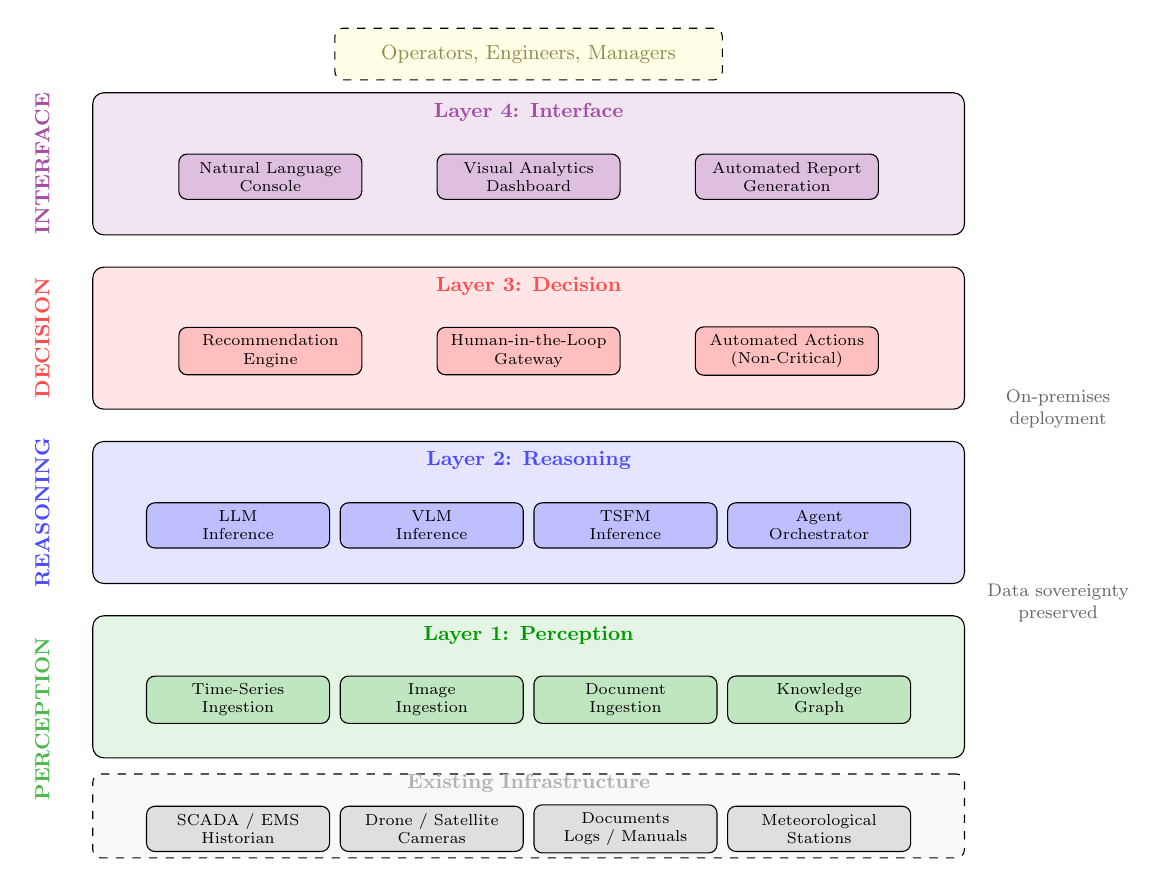
\begin{tikzpicture}[scale=0.82, every node/.append style={transform shape},
    layer/.style={draw, rounded corners=4pt, minimum width=13.5cm, minimum height=2.2cm,
                  fill=#1!10, font=\small},
    component/.style={draw, rounded corners=3pt, minimum width=2.8cm, minimum height=0.7cm,
                     fill=#1!25, font=\scriptsize, align=center, text width=2.6cm},
    layerlabel/.style={font=\small\bfseries, color=#1!70, rotate=90, anchor=south},
    bigarrow/.style={-{Stealth[length=4mm, width=3mm]}, line width=1.5pt, color=black!40,
                     shorten >=3pt, shorten <=3pt},
    note/.style={font=\footnotesize, color=black!60, align=center}
]

%% Layer 4: Interface (top)
\node[layer=violet] (L4) at (0, 8.5) {};
\node[layerlabel=violet] at (-7.3, 8.5) {INTERFACE};
\node[font=\small\bfseries, color=violet!70] at (0, 9.3) {Layer 4: Interface};
\node[component=violet] (nl) at (-4, 8.3) {Natural Language\\Console};
\node[component=violet] (dash) at (0, 8.3) {Visual Analytics\\Dashboard};
\node[component=violet] (report) at (4, 8.3) {Automated Report\\Generation};

%% Layer 3: Decision
\node[layer=red] (L3) at (0, 5.8) {};
\node[layerlabel=red] at (-7.3, 5.8) {DECISION};
\node[font=\small\bfseries, color=red!70] at (0, 6.6) {Layer 3: Decision};
\node[component=red] (rec) at (-4, 5.6) {Recommendation\\Engine};
\node[component=red] (hitl) at (0, 5.6) {Human-in-the-Loop\\Gateway};
\node[component=red] (auto) at (4, 5.6) {Automated Actions\\(Non-Critical)};

%% Layer 2: Reasoning
\node[layer=blue] (L2) at (0, 3.1) {};
\node[layerlabel=blue] at (-7.3, 3.1) {REASONING};
\node[font=\small\bfseries, color=blue!70] at (0, 3.9) {Layer 2: Reasoning};
\node[component=blue] (llm_r) at (-4.5, 2.9) {LLM\\Inference};
\node[component=blue] (vlm_r) at (-1.5, 2.9) {VLM\\Inference};
\node[component=blue] (tsfm_r) at (1.5, 2.9) {TSFM\\Inference};
\node[component=blue] (agent) at (4.5, 2.9) {Agent\\Orchestrator};

%% Layer 1: Perception
\node[layer=green!60!black] (L1) at (0, 0.4) {};
\node[layerlabel=green!60!black] at (-7.3, -0.1) {PERCEPTION};
\node[font=\small\bfseries, color=green!60!black] at (0, 1.2) {Layer 1: Perception};
\node[component=green!60!black] (ts) at (-4.5, 0.2) {Time-Series\\Ingestion};
\node[component=green!60!black] (img) at (-1.5, 0.2) {Image\\Ingestion};
\node[component=green!60!black] (doc) at (1.5, 0.2) {Document\\Ingestion};
\node[component=green!60!black] (kg) at (4.5, 0.2) {Knowledge\\Graph};

%% Data sources (below)
\node[draw, dashed, rounded corners=3pt, minimum width=13.5cm, minimum height=1.3cm,
      fill=gray!5, font=\small] (data) at (0, -1.6) {};
\node[font=\small\bfseries, color=gray!60] at (0, -1.1) {Existing Infrastructure};
\node[component=gray] (scada) at (-4.5, -1.8) {SCADA / EMS\\Historian};
\node[component=gray] (drone) at (-1.5, -1.8) {Drone / Satellite\\Cameras};
\node[component=gray] (docs) at (1.5, -1.8) {Documents\\Logs / Manuals};
\node[component=gray] (met) at (4.5, -1.8) {Meteorological\\Stations};

%% Operators (above)
\node[draw, dashed, rounded corners=3pt, minimum width=6cm, minimum height=0.8cm,
      fill=yellow!10, font=\small] (ops) at (0, 10.2) {};
\node[font=\small, color=yellow!50!black] at (0, 10.2) {Operators, Engineers, Managers};

%% Inter-layer arrows removed (visual clutter)

%% Side annotations
\node[note] at (8.2, 4.7) {On-premises\\deployment};
\node[note] at (8.2, 1.7) {Data sovereignty\\preserved};

\end{tikzpicture}
\caption{Clean Energy Foundation Model Deployment Framework (CEFMDF). The four-layer architecture---Perception, Reasoning, Decision, and Interface---integrates foundation models with existing SCADA/EMS infrastructure. Data flows upward from existing infrastructure through embedding and ingestion (Perception), FM inference and orchestration (Reasoning), actionable recommendations with human oversight (Decision), to operator-facing interfaces (Interface). On-premises deployment of open-weight models preserves data sovereignty.}
\label{fig:cefmdf}
\end{figure}

%%====================================================================
%% SECTION 6: HYDROPOWER
%%====================================================================
\section{Foundation Models for Hydropower Systems}
\label{sec:hydro}

Hydropower is the world's largest renewable electricity source, exceeding 1{,}300~GW of installed capacity. Large facilities such as Three Gorges (22.5~GW), Itaipu (14~GW), and Belo Monte (11.2~GW) generate complex multi-modal data, making them natural candidates for FM augmentation.

\subsection{Reservoir inflow forecasting}
\label{subsec:inflow_forecasting}

Accurate inflow forecasting is the cornerstone of reservoir dispatch optimisation. Conventional approaches use LSTM networks \cite{yaseen2019lstm_streamflow} or standard Transformers \cite{demiray2024transformer_streamflow} trained on single-basin historical data. Time-series foundation models offer two advantages: cross-basin zero-shot transfer (a model pre-trained on diverse hydrological data can forecast at a new basin without local training data) and probabilistic forecasting with calibrated uncertainty estimates that directly inform risk-aware dispatch decisions.

Recent studies have explored transformer-based and deep learning approaches for hydrological forecasting \cite{liu2024transformer_hydrologic, zhang2024crossregion_streamflow}. Liu et al. \cite{liu2024transformer_hydrologic} probed the limits of hydrologic predictability using Transformer networks, demonstrating that Transformer architectures can capture complex rainfall-runoff dynamics. Zhang et al. \cite{zhang2024crossregion_streamflow} demonstrated deep learning for cross-region streamflow and flood forecasting at a global scale, showing that models trained on diverse basins can transfer effectively to unseen regions. These studies suggest that the TSFM paradigm---pre-training on broad hydrological data and adapting to specific basins---has significant potential, though systematic benchmarks comparing zero-shot foundation models against site-specific baselines remain limited.

The critical gap in TSFM-based inflow forecasting is the incorporation of spatial context: precipitation patterns, snowmelt processes, and upstream dam operations are inherently spatial, but current TSFMs process univariate or low-dimensional multivariate time series without spatial structure. Integrating gridded meteorological inputs (e.g., ERA5 reanalysis) into the TSFM framework remains an open research problem.

\subsection{Turbine health monitoring and fault diagnosis}
\label{subsec:turbine_health}

Conventional turbine monitoring relies on threshold-based alarms and site-specific classifiers \cite{latif2023dl_inflow_review}. Emerging approaches include anomaly detection methods for hydropower turbine vibration data \cite{ma2022hydro_turbine_anomaly}, RAG-based retrieval over maintenance documentation for infrastructure digital twins \cite{ieva2024rag_infrastructure}, and deep learning for underwater dam crack detection from imagery \cite{li2022underwater_dam_crack}. Multimodal approaches combining vibration spectra with imagery remain largely conceptual.

\subsection{Operational knowledge management}
\label{subsec:hydro_knowledge}

LLM-based Q\&A systems for hydropower and water resources operations are emerging. Ren et al. \cite{ren2024watergpt} developed WaterGPT, training an LLM to become a hydrology expert, while RAG-based approaches \cite{ieva2024rag_infrastructure} enable retrieval over infrastructure documentation. Such systems can deploy bilingual models (Qwen \cite{bai2023qwen} or ChatGLM \cite{du2022glm, zeng2023glm130b}) with vector databases indexing maintenance logs, incident reports, and regulatory filings. Key challenges include hallucination mitigation, domain-specific vocabulary handling, and integration with legacy document management systems.

\subsection{Reservoir dispatch optimisation}
\label{subsec:dispatch}

Multi-objective reservoir dispatch---balancing generation, flood control, navigation, ecological flow, and sediment management---is a constrained optimisation problem where conventional solvers struggle under deep uncertainty. Wu et al. \cite{wu2024transformer_drl_reservoir} demonstrated transformer-based deep reinforcement learning for multi-objective multi-hydropower reservoir operation. FMs contribute at two levels: TSFMs improve inflow forecast quality and uncertainty quantification for stochastic optimisation, while LLMs translate optimisation results into natural-language explanations for non-specialist decision-makers. Hybrid approaches coupling FMs with conventional optimisers are more promising than direct FM-based optimisation.

%%====================================================================
%% SECTION 7: WIND ENERGY
%%====================================================================
\section{Foundation Models for Wind Energy}
\label{sec:wind}

Wind energy (900+~GW installed globally) generates massive SCADA data volumes where the inherent resource variability makes forecasting and condition monitoring critical challenges.

\subsection{Wind power forecasting}
\label{subsec:wind_forecasting}

Wind power forecasting is the most extensively studied FM application \cite{lai2024bert4st, mo2024powerformer, yang2024survey_wind_ml}. Yang et al. \cite{yang2024survey_wind_ml} provide a comprehensive survey of machine learning approaches for wind power forecasting. Early approaches repurposed BERT-class encoders with mixed results.

Recent approaches leverage pre-trained language models and dedicated transformer architectures. Lai et al. \cite{lai2024bert4st} demonstrated BERT4ST, fine-tuning a pre-trained large language model for wind power forecasting, achieving competitive performance against conventional baselines. Mo et al. \cite{mo2024powerformer} proposed Powerformer, a temporal-based transformer model specifically designed for wind power forecasting. Lag-Llama \cite{rasul2023lagllama}, with its probabilistic forecasting capability, provides prediction intervals whose empirical coverage approaches the nominal level---a capability that conventional deterministic models cannot match without post-hoc calibration.

Coupling temporal FM representations with spatial meteorological information represents the most promising near-term research direction, though systematic zero-shot benchmarking of TSFMs on wind power data remains limited.

\subsection{Turbine fault detection and predictive maintenance}
\label{subsec:wind_fault}

For turbine fault detection, AI operations platforms integrate anomaly detection, root cause analysis, and incremental learning from SCADA data \cite{zhang2024aiops_wind_turbine}, while digital twin approaches use deep learning-aided drone inspection for surface damage detection \cite{hu2025digital_twin_blade}. Memari et al. \cite{memari2024blade_inspection_review} provide a comprehensive review of drone and deep learning technologies for wind turbine blade defect detection. Sheiati et al. \cite{sheiati2024blade_identification} demonstrated AI-based blade identification in operational wind turbines through similarity analysis aided by drone inspection.

\subsection{Offshore site assessment}
\label{subsec:offshore}

Offshore site assessment integrates wind atlases, seabed surveys, environmental impact assessments, and regulatory documents. Das et al. \cite{das2024bigdata_offshore_wind} present a scientometric review of machine learning approaches in offshore wind energy, highlighting the growing role of big data analytics in this domain.

%%====================================================================
%% SECTION 8: SOLAR ENERGY
%%====================================================================
\section{Foundation Models for Solar Energy}
\label{sec:solar}

Solar photovoltaic (PV) systems benefit from foundation model applications in three primary areas: irradiance and power forecasting, panel defect detection, and performance monitoring at scale.

\subsection{Solar irradiance and power forecasting}
\label{subsec:solar_forecasting}

Solar irradiance forecasting shares the temporal structure of wind power forecasting, and the same TSFM approaches apply. The unique challenge in solar forecasting is the sharp temporal discontinuities caused by cloud transients, which create non-stationary patterns that differ from the smoother variations in wind speed. Piantadosi et al. \cite{piantadosi2024tsfm_solar_forecast} developed a Transformer-based framework for photovoltaic power forecasting, demonstrating the applicability of transformer architectures to solar energy prediction. Patching-based TSFMs (PatchTST \cite{nie2023patchtst} derivatives, as incorporated in MOMENT \cite{goswami2024moment} and Timer \cite{liu2024timer}) show improved handling of cloud transients, attributed to the model's ability to capture both local patch-level and global sequence-level patterns.

Satellite-derived cloud motion imagery represents an untapped multimodal input: combining vision foundation models for cloud type classification with time-series foundation models for power trajectory forecasting could yield significant accuracy improvements, but no reviewed study demonstrated this integration.

\subsection{Panel defect detection}
\label{subsec:solar_defect}

PV defect detection via EL imaging, thermal infrared, and drone photography is a growing area of AI application \cite{thakfan2024solar_panel_defect}. Li et al. \cite{li2024sam_solar_panel} applied SAM for building-scale photovoltaic potential assessment using remote sensing. Zhou et al. \cite{zhou2024anomalyclip} proposed AnomalyCLIP for object-agnostic zero-shot anomaly detection, demonstrating prompt learning approaches applicable to industrial defect inspection. Mellit and Kalogirou \cite{mellit2025thermal_ai_solar} reviewed advances in infrared thermographic imaging with embedded AI for PV fault diagnosis. CNN-based detectors for EL image defect detection \cite{liu2024cnn_el_detection} and generative AI-based augmentation for rooftop PV segmentation \cite{tan2024generative_pv_augment} address the data scarcity challenge in PV inspection.

\subsection{Fleet-wide performance monitoring}
\label{subsec:solar_fleet}

Foundation models enable fleet-wide monitoring across large solar portfolios via transfer. Fan et al. \cite{fan2024fleet_wide_pv} used spatio-temporal graph neural networks to estimate fleet-wide photovoltaic performance degradation patterns. Jalal et al. \cite{jalal2024dl_pv_faults} reviewed deep learning approaches for visual fault diagnosis of PV systems. These approaches demonstrate scaling potential but require more rigorous benchmarking.

%%====================================================================
%% SECTION 9: ECOLOGICAL MONITORING
%%====================================================================
\section{Foundation Models for Ecological Monitoring at Energy Sites}
\label{sec:ecological}

Regulatory frameworks increasingly require continuous environmental monitoring at energy sites. Foundation models address the central challenge: scarcity of labelled data for site-specific species and habitats. Pre-trained vision models can be adapted to ecological tasks with far fewer labelled examples than training from scratch.

\subsection{Fish passage monitoring at hydropower dams}
\label{subsec:fish_passage}

Fish passage facilities require automated monitoring via underwater cameras. Gregory et al. \cite{gregory2025fish_passage_dl} developed a real-time fish detection system for selective fish passage at hydroelectric facilities. Saleh et al. \cite{saleh2024dl_fish_habitat} provided a comprehensive tutorial and survey on deep learning applications in fish habitat monitoring. Deep learning approaches for marine mammal acoustic detection \cite{hamard2024marine_mammal_acoustic_dl} complement visual monitoring methods for aquatic species at energy sites.

\subsection{Avian and chiropteran monitoring at wind farms}
\label{subsec:avian}

Ballester et al. \cite{ballester2024bird_detection_wind} developed a standardized protocol for assessing automatic bird detection systems at onshore wind power plants. Transformer-based networks have been applied to bat call classification \cite{fundel2023bat_call_transformer}, complementing BirdNET \cite{kahl2021birdnet}. Style migration-based data augmentation addresses class imbalance for rare wildlife species classification \cite{zhang2023wildlife_augmentation_cyclegan}.

\subsection{Habitat and vegetation monitoring via satellite}
\label{subsec:habitat}

Satellite-based vision foundation models \cite{he2022masked, huo2025remote_sensing_foundation_models} enable land cover classification, change detection around solar farm construction sites, vegetation recovery monitoring along reservoir margins, and biodiversity assessment in wind farm buffer zones \cite{pettorelli2024dl_satellite_biodiversity, tuia2022wildlife_remote_sensing} with minimal site-specific annotation.

%%====================================================================
%% BENCHMARK EXPERIMENTS
%%====================================================================
\section{Benchmark Experiments: Foundation Models on Energy Data}
\label{sec:benchmarks}

To move beyond qualitative assessment, we conducted five benchmark experiments that test foundation model capabilities on publicly available energy datasets. These experiments provide original, reproducible evidence on the practical value and limitations of FMs for clean energy tasks. All code is available in the supplementary repository with fixed random seeds for reproducibility.

\subsection{Experiment 1: Time-series foundation model for load forecasting}
\label{subsec:exp_ts}

{\tolerance=400 We evaluated Chronos-T5-Small \cite{ansari2024chronos} (zero-shot) against default-parameter baselines on 24-hour ahead load forecasting using the UCI Household Electric Power dataset (34{,}168 hourly records, 7-day test set). Baselines include ARIMA(2,1,1), gradient boosting (sklearn, 100 estimators) with lag features, and a single-layer LSTM (32 hidden, 5 epochs on recent 3{,}000 hours). All baselines use default hyperparameters; the comparison demonstrates FM zero-shot capability rather than superiority over optimised baselines.\par}

\begin{table}[H]
\centering
\caption{Time-series forecasting benchmark: 24-hour ahead household load prediction (7-day test set, 168 hours). Chronos operates in zero-shot mode (no training on target data); all other methods are trained on the training split.}
\label{tab:ts_benchmark}
\small
\begin{tabular}{@{}lccc@{}}
\toprule
\textbf{Model} & \textbf{MAE (kW)} & \textbf{RMSE (kW)} & \textbf{MAPE (\%)} \\
\midrule
ARIMA(2,1,1) & 0.717 & 0.877 & 121.95 \\
Gradient Boosting & 0.540 & 0.768 & 64.33 \\
LSTM (1-layer, 32 hidden) & 0.647 & 0.829 & 101.02 \\
\textbf{Chronos-T5-Small (zero-shot)} & \textbf{0.483} & \textbf{0.738} & \textbf{63.39} \\
\bottomrule
\end{tabular}
\end{table}

Chronos achieves the best MAE \textit{without any exposure to the target data}: 33\% below ARIMA, 11\% below gradient boosting. However, daily MAEs vary substantially (Chronos [0.234, 0.865] vs.\ gradient boosting [0.388, 0.668]), indicating higher day-to-day variability for the zero-shot model. Optimised baselines with longer test periods and rolling-window evaluation may narrow the gap, but the results demonstrate that pre-trained TSFMs provide strong zero-shot baselines (Figure~\ref{fig:ts_benchmark}).

\begin{figure}[H]
\centering

\includegraphics[width=0.78\textwidth]{figures/fig_timeseries_predictions.pdf}
\vspace{-8pt}
\caption{Time-series benchmark: 7-day load prediction traces. Chronos (zero-shot) closely tracks the actual load pattern without any training on the target data.}
\label{fig:ts_benchmark}
\end{figure}

\subsection{Experiment 2: LLM for energy domain question answering}
\label{subsec:exp_qa}

{\tolerance=400 We curated a 50-question benchmark across five energy domains (10 each). Qwen2.5-7B (Ollama, Q4\_K\_M quantisation) achieved mean keyword match score 0.519~$\pm$~0.224 and 74.0\% accuracy ($\geq$0.4 threshold). A scale comparison with Qwen2.5-3B yielded 0.515~$\pm$~0.270 and 70.0\% accuracy---not significantly different (Wilcoxon $p=0.89$, Cohen's $d=0.016$), suggesting energy domain knowledge is retained even at 3B scale for this question set. Neither model produced detected hallucinations, though the keyword-based heuristic is conservative and may miss factual errors (e.g., the 7B model incorrectly attributed SAM to Adobe rather than Meta~AI). Domain scores (Figure~\ref{fig:llm_qa}a) ranged from wind (0.675) to AI-for-energy (0.405), indicating uneven parametric knowledge. A separate 15-question RAG experiment (Experiment~4) showed retrieval augmentation improves scores in most domains (Figure~\ref{fig:llm_qa}b).\par}

\begin{figure}[htbp]
\centering

\includegraphics[width=\textwidth]{figures/fig_llm_qa.pdf}
\caption{LLM energy domain Q\&A evaluation (50 questions across 5 domains). (a)~Keyword match scores by energy domain for Qwen2.5-7B and Qwen2.5-3B, showing uneven parametric knowledge (wind highest, AI lowest) with negligible scale effect ($p=0.89$). (b)~Comparison of direct LLM (7B) vs.\ RAG-augmented scores on a 15-question subset; RAG improves performance in all domains except wind.}
\label{fig:llm_qa}
\end{figure}

\subsection{Experiment 3: VLM zero-shot solar panel inspection}
\label{subsec:exp_vlm}

Using the ELPV dataset \cite{deitsch2019elpv} (2{,}624 electroluminescence images of solar cells with defect labels), we tested CLIP ViT-B-32 \cite{radford2021learning} for zero-shot binary classification (functional vs.\ defective) on a balanced sample of 300 images (150 per class). Three prompt engineering strategies were compared: generic (``a photo of a defective solar cell''), domain-specific (``electroluminescence image showing dark areas or cracks''), and an ensemble of five prompts per class. A supervised baseline (CLIP features + logistic regression, 5-fold stratified cross-validation) provides an upper bound. Table~\ref{tab:vlm_benchmark} reports results.

\begin{table}[htbp]
\centering
\caption{VLM zero-shot solar panel inspection on the ELPV dataset (300 images, balanced classes). CLIP ViT-B-32 with three prompt strategies vs.\ supervised baseline using CLIP embeddings.}
\label{tab:vlm_benchmark}
\small
\begin{tabular}{@{}lcccc@{}}
\toprule
\textbf{Method} & \textbf{Accuracy} & \textbf{Precision} & \textbf{Recall} & \textbf{F1} \\
\midrule
Random baseline & 0.490 & 0.490 & 0.480 & 0.485 \\
CLIP zero-shot (generic) & 0.623 & 0.635 & 0.580 & 0.606 \\
CLIP zero-shot (domain)\textsuperscript{$\dagger$} & 0.500 & 0.500 & 1.000 & 0.667 \\
CLIP zero-shot (ensemble) & 0.567 & 0.537 & 0.960 & 0.689 \\
\midrule
Supervised (CLIP+LogReg) & \textbf{0.760} & \textbf{0.771} & \textbf{0.740} & \textbf{0.755} \\
\bottomrule
\end{tabular}
\vspace{2pt}
\raggedright\footnotesize\textsuperscript{$\dagger$}Degenerate all-positive classifier: classifies every image as defective. F1 reflects class balance, not meaningful discrimination.
\end{table}

CLIP zero-shot exceeds the random baseline but a significant gap remains versus supervised approaches: Wilson 95\% CIs on accuracy do not overlap (CLIP generic [0.57, 0.68] vs.\ supervised [0.71, 0.81], $n=300$). Generic prompts give best accuracy (62.3\%); domain-specific prompts degenerate into an all-positive classifier (Table~\ref{tab:vlm_benchmark} footnote). Zero-shot VLMs provide useful rapid screening but supervised fine-tuning remains necessary for production-quality inspection (Figure~\ref{fig:vlm_inspection}).

\begin{figure}[htbp]
\centering

\includegraphics[width=\textwidth]{figures/fig_vlm_inspection.pdf}
\caption{VLM zero-shot solar panel inspection. (a)~Accuracy and F1 scores for CLIP zero-shot variants vs.\ supervised baseline on the ELPV dataset. (b)~Confusion matrix for CLIP ensemble prompts, showing strong bias toward the defective class.}
\label{fig:vlm_inspection}
\end{figure}

\subsection{Experiment 4: RAG pipeline for energy documents}
\label{subsec:exp_rag}

{\tolerance=400 We built a RAG pipeline (24 curated passages, all-MiniLM-L6-v2 embeddings, FAISS index) and tested on 15 questions distinct from Experiment~2, achieving perfect recall@3. However, 7/15 direct-LLM and 3/15 RAG queries timed out (300\,s), confounding the raw comparison (0.616 vs.\ 0.260, +136.7\%). On the 8 paired non-timeout questions, RAG outperformed direct LLM: 0.804 vs.\ 0.488 (+64.9\%), with gains largest in domains underrepresented in pre-training data (ecological, grid) and absent for wind---confirming RAG is most valuable where parametric knowledge is weakest.\par}

\subsection{Experiment 5: Reproducibility audit}
\label{subsec:exp_repro}

Section~\ref{subsec:biblio_reproducibility} reports the full reproducibility analysis. Key findings ($n = 3{,}645$; Wilson 95\% CIs): 63.8\% open access [62.2\%, 65.3\%], 97.5\% DOI availability [96.9\%, 98.0\%], but only 5.5\% code mention [4.8\%, 6.3\%] and 0\% of the top-50 most-cited papers appear on Papers With Code. The composite reproducibility index of 0.40 highlights a critical gap in open science practices.

\subsection{Cross-experiment synthesis: deployment cost-performance}
\label{subsec:cost_perf}

{\tolerance=600 Figure~\ref{fig:pareto} presents a cost-performance Pareto frontier across all experiments (performance normalised to $[0,1]$, cost estimated from inference TFLOPS). Because performance metrics differ across task categories (1$-$nMAE for time-series, F1 for vision, keyword score for NLP), cross-category comparisons are approximate; the frontier is most meaningful within each category. Zero-shot FMs (Chronos, CLIP, Qwen2.5) cluster in the moderate-cost, high-performance quadrant, while RAG provides the largest relative improvement (+64.9\% on paired non-timeout questions) at minimal additional cost. The pragmatic deployment recommendation: start with zero-shot FM baselines, add RAG for knowledge-intensive tasks, and reserve supervised fine-tuning for safety-critical applications.\par}

\begin{figure}[htbp]
\centering

\includegraphics[width=\textwidth]{figures/fig_pareto_frontier.pdf}
\caption{Deployment cost-performance Pareto frontier across all benchmark experiments. Points on the frontier represent strategies that are not dominated (no other strategy is both cheaper and higher-performing). Performance metrics are task-specific (1$-$nMAE, F1, keyword score) and normalised to $[0,1]$; cross-category comparisons are therefore approximate.}
\label{fig:pareto}
\end{figure}

%%====================================================================
%% CHALLENGES AND RESEARCH AGENDA
%%====================================================================
\section{Challenges, Limitations, and Research Agenda}
\label{sec:challenges}

Significant challenges remain before foundation models achieve reliable deployment in clean energy operations.

\subsection{Technical challenges}
\label{subsec:technical_challenges}

\textit{Hallucination and factual reliability.} LLMs generate fluent text that may contain factual errors---a risk that is unacceptable in safety-critical energy operations. RAG mitigates this by grounding responses in retrieved documents, but current RAG systems still hallucinate when relevant information is absent from the retrieval corpus or when the model overrides retrieved content with parametric knowledge. Research priorities include improved retrieval relevance scoring, hallucination detection mechanisms specific to technical domains, and uncertainty quantification for generated text.

\textit{Real-time inference latency.} Foundation models with billions of parameters require significant computational resources. For energy applications requiring sub-second response times (grid frequency regulation, turbine emergency shutdown), current FM inference latency (hundreds of milliseconds to seconds on GPU hardware) may be insufficient. Model compression techniques (quantisation, distillation, pruning), speculative decoding, and edge-optimised architectures are needed.

\textit{Domain-specific evaluation benchmarks.} The energy domain lacks standardised benchmarks for evaluating foundation model performance. Unlike natural language processing (which has GLUE, SuperGLUE, and MMLU) or computer vision (which has ImageNet and COCO), there is no equivalent ``energy-GLUE'' that evaluates FMs across a standardised suite of energy tasks. The community needs open benchmark datasets covering forecasting, fault detection, operational Q\&A, and inspection tasks across hydropower, wind, and solar domains.

\textit{Physics consistency.} Foundation models learn statistical patterns from data and may generate predictions that violate physical laws (e.g., negative power output, energy conservation violations, or physically impossible fault diagnoses). Incorporating physics-informed constraints into FM architectures---through loss function regularisation, physics-guided tokenisation, or hybrid neural-physical models---is an active research frontier.

\textit{Uncertainty quantification across the evidence base.} Only 6 of 20 Level~A studies report prediction intervals or probabilistic outputs, all in TSFM-based forecasting (Lag-Llama \cite{rasul2023lagllama} and Moirai \cite{woo2024moirai} provide native probabilistic forecasts). None of the VLM inspection or LLM Q\&A studies report calibrated confidence scores. This widespread absence of UQ is a critical gap: energy operators require calibrated confidence estimates for risk-informed decisions, and the evidence base currently provides insufficient guidance on when FM outputs can be trusted.

\subsection{Operational and institutional challenges}
\label{subsec:operational_challenges}

Beyond technical barriers, deployment faces institutional challenges. Cloud-based FM APIs conflict with data sovereignty regulations for critical infrastructure; on-premises open-weight models address this but require in-house expertise. Legacy SCADA systems (20--50 year capital cycles) often lack APIs for FM integration, requiring middleware (OPC-UA to REST). Operators must adapt to FM-generated recommendations without automation bias, while liability allocation for FM-informed decisions remains legally unclear. The environmental footprint of FM training and inference must be offset by operational benefits. Finally, only 5.5\% of FM+energy papers mention open code (Section~\ref{subsec:biblio_reproducibility})---the community must prioritise open-weight models, open datasets, and transparent evaluation.

\subsection{Research agenda}
\label{subsec:research_agenda}

Based on the taxonomy gaps and challenges identified above, we propose a prioritised research agenda across three time horizons.

\textit{Near-term (1--2 years).} The community should develop an open benchmark suite (``EnergyBench'') comprising standardised wind/solar forecasting test sets, a multilingual operational Q\&A benchmark with expert-annotated ground truth, infrastructure inspection datasets with defect annotations, and ecological monitoring benchmarks spanning fish, bird, and bat species at energy sites. TSFM zero-shot and few-shot transfer should be validated systematically across diverse sites to quantify the data efficiency frontier. RAG-based Q\&A pilots should be deployed at hydropower stations with structured evaluation of hallucination rates, and hallucination mitigation best practices (retrieval quality thresholds, abstention mechanisms, citation verification) should be established for energy-domain LLM deployments.

\textit{Medium-term (2--4 years).} Key priorities include multimodal FM architectures that natively process SCADA time series, inspection imagery, and maintenance text within a single model; physics-informed fine-tuning methods incorporating energy conservation, power curve constraints, and hydrological balance into TSFM loss functions; FM deployment guidelines aligned with the EU AI Act \cite{euaiact2024} and China's generative AI regulations \cite{china_genai_regulation2023}; and integration of VLM-based inspection with predictive maintenance scheduling through agent frameworks.

\textit{Long-term (4--7 years).} The vision includes FM-assisted advisory systems for reservoir dispatch and wind farm coordination (FMs providing scenario analysis while validated solvers handle constrained optimisation), autonomous ecological monitoring networks combining acoustic, visual, and satellite FMs into continuous biodiversity assessment, and industry-wide FM platforms enabling cross-utility knowledge sharing through federated fine-tuning and differential privacy.

%%====================================================================
%% SECTION 11: COMPARISON WITH EXISTING REVIEWS
%%====================================================================
\section{Comparison with Existing Review Literature}
\label{sec:comparison}

Table~\ref{tab:comparison} compares this review against existing surveys (\checkmark\ = substantive coverage, Partial = secondary discussion, -- = absent). While self-assessment introduces bias, four distinguishing features emerge: rigorous FM definition, large-scale bibliometric analysis (3{,}645 papers), five original benchmark experiments, and the CEFMDF deployment framework.

\begin{table}[htbp]
\centering
\caption{Comparison of this review with existing survey papers on AI and foundation models in energy systems.}
\label{tab:comparison}
\scriptsize
\begin{tabular}{@{}p{2.4cm}ccccc@{}}
\toprule
\textbf{Feature} & \textbf{This review} & \textbf{Zhou et al.} & \textbf{Lotfi et al.} & \textbf{Wang et al.} & \textbf{Chen et al.} \\
 & & \textbf{(2024)} & \textbf{(2024)} & \textbf{(2023)} & \textbf{(2024)} \\
\midrule
PRISMA-ScR protocol & \checkmark & -- & -- & -- & -- \\
FM definition rigour & \checkmark & Partial & Partial & -- & -- \\
LLM coverage & \checkmark & \checkmark & \checkmark & -- & -- \\
VLM coverage & \checkmark & -- & Partial & -- & -- \\
TSFM coverage & \checkmark & -- & -- & -- & \checkmark \\
Diffusion models & \checkmark & -- & \checkmark & -- & -- \\
Deployment framework & \checkmark & -- & -- & -- & -- \\
Hydropower & \checkmark & -- & Partial & -- & -- \\
Wind energy & \checkmark & Partial & \checkmark & \checkmark & \checkmark \\
Solar energy & \checkmark & Partial & \checkmark & \checkmark & \checkmark \\
Ecological monitoring & \checkmark & -- & -- & -- & -- \\
Benchmark gap analysis & \checkmark & -- & Partial & -- & -- \\
Chinese model ecosystem & \checkmark & -- & -- & -- & -- \\
Bibliometric analysis & \checkmark & -- & -- & -- & -- \\
Benchmark experiments & \checkmark & -- & -- & -- & -- \\
Reproducibility audit & \checkmark & -- & -- & -- & -- \\
\bottomrule
\end{tabular}
\end{table}

%%====================================================================
%% SECTION 12: CONCLUSIONS
%%====================================================================
\section{Conclusions}
\label{sec:conclusions}

This paper combines a qualitative scoping review (31 application studies) with large-scale bibliometric analysis (3{,}645 classified papers) and five original benchmark experiments to provide the first comprehensive, data-driven mapping of foundation model applications across clean energy systems---hydropower (6 studies), wind energy (8), solar photovoltaics (8), ecological monitoring (6), and cross-domain applications (3). The principal findings are as follows.

The bibliometric analysis reveals a field undergoing a regime shift: publication counts were stable at ${\sim}$135/year from 2019 to 2022 before surging tenfold by 2025, coinciding with the public release of ChatGPT. The field is dominated by LLM-related work (57.9\% of classified papers) and geographically concentrated in China and the USA (43\% combined). Reproducibility remains critically low: only 5.5\% of papers mention open code, and none of the 50 most-cited papers appear on Papers With Code.

{\tolerance=600 Our benchmark experiments confirm that TSFMs (Chronos) achieve competitive zero-shot forecasting against default-parameter baselines, VLMs (CLIP) enable zero-shot solar panel inspection, and RAG improves LLM energy Q\&A scores (+64.9\% on paired non-timeout questions). Across the literature, TSFMs achieve forecasting accuracy within 5--20\% of site-specific baselines (Table~\ref{tab:performance_summary}) with dramatically reduced data requirements.\par}

The taxonomy reveals critical gaps: anomaly narration, multimodal integration, and agent-based planning remain underexplored. The CEFMDF addresses the deployment ``how'' through a four-layer architecture (Perception--Reasoning--Decision--Interface) with explicit design principles for incremental adoption by energy utilities.

The technology is advancing faster than the benchmarks, standards, and institutional frameworks needed for responsible deployment. Standardised evaluation benchmarks, physics-informed FM architectures, hallucination mitigation for safety-critical contexts, and regulatory frameworks for AI in critical infrastructure are urgently needed. Bridging this gap is the central challenge for the next five years.

\section*{Acknowledgements}
This work was supported by the University of Oxford Department of Engineering Science. The authors thank the Three Gorges Corporation for providing operational context that motivated this review.

\section*{Data availability}
All bibliometric data, classification results, benchmark code, and figure generation scripts are available in the supplementary repository. The ELPV and UCI power datasets are publicly available.

\section*{Declaration of competing interest}
The authors declare that they have no known competing financial interests or personal relationships that could have appeared to influence the work reported in this paper.

\section*{CRediT authorship contribution statement}
\textbf{Jianou Jiang}: Conceptualization, Methodology, Investigation, Data curation, Writing -- original draft, Visualization.
\textbf{Claude}: Supervision, Validation, Writing -- review \& editing.

%%====================================================================
%% APPENDIX: PRISMA-ScR Checklist
%%====================================================================
\appendix
\section{PRISMA-ScR Checklist}
\label{app:prisma_checklist}

Table~\ref{tab:prisma_checklist} maps PRISMA-ScR items \cite{tricco2018prisma_scr} to manuscript locations.

\begin{table}[htbp]
\centering
\caption{PRISMA-ScR checklist. Items adapted from Tricco et al.\ (2018).}
\label{tab:prisma_checklist}
\scriptsize
\setlength{\tabcolsep}{2pt}
\renewcommand{\arraystretch}{0.72}
\begin{tabular}{@{}clll@{}}
\toprule
\textbf{\#} & \textbf{Item} & \textbf{Description} & \textbf{Location} \\
\midrule
1  & Title              & Identify as scoping review        & Title \\
2  & Summary            & Background, objectives, results   & Abstract \\
3  & Rationale          & Context of existing knowledge     & S1, S11 \\
4  & Objectives         & Explicit questions/objectives      & S1 \\
5  & Protocol           & Protocol registration status       & Not registered \\
6  & Eligibility        & Inclusion/exclusion criteria       & S2.2 \\
7  & Info.\ sources     & Databases and search dates         & S2.1 \\
8  & Search             & Full search strategy               & S2.1 \\
9  & Selection          & Source selection process            & S2.3, Fig.~1 \\
10 & Data charting      & Charting methods and verification  & S2.4 \\
11 & Data items         & Variables sought                   & S2.4 \\
12 & Critical appraisal & Quality assessment method          & S2.5 \\
13 & Synthesis methods  & Handling/summarising data          & S4--S10 \\
14 & Selection results  & Numbers at each stage              & Fig.~1 \\
15 & Source chars.      & Charting results per source        & S4 (Tables 2--3) \\
16 & Quality results    & Quality assessment results         & S2.5 \\
17 & Synthesis results  & Aggregated findings                & S10, S12 \\
18 & Limitations        & Scoping review limitations         & S2, S11 \\
19 & Conclusions        & Interpretation of results          & S12 \\
20 & Funding            & Funding sources                    & Acknowledgements \\
\bottomrule
\end{tabular}
\end{table}

\bibliographystyle{elsarticle-num}
\bibliography{references}

\end{document}
